
\NeedsTeXFormat{LaTeX2e}
\documentclass[12pt]{article}

\usepackage{titlesec}
\usepackage{setspace}
\usepackage{amsmath}
\usepackage{amssymb}
\usepackage{epsfig}
\usepackage{fancybox}
\usepackage{listings}
%\usepackage{algo}
\usepackage{url}
\usepackage{xcolor}
\usepackage{adjustbox}
\usepackage{float}
\usepackage{multicol}
\usepackage[utf8]{inputenc}
\usepackage[colorlinks=true,linkcolor=blue]{hyperref}

\newcommand{\phil}[1]{{\color{red}(\textbf{Phil:} #1)}}
\newcommand{\yue}[1]{{\color{blue}(\textbf{Yue:} #1)}}
\newcommand{\specialcell}[2][c]{%
	\begin{tabular}[#1]{@{}c@{}}#2\end{tabular}}


\setlength{\textheight}{9in}
\setlength{\textwidth}{6in}
\setlength{\oddsidemargin}{.25in}
\setlength{\topmargin}{-.5in}  % changed from -.25 by RSR on 1/21/07
%\parindent .5in    % commented out by RSR 1/21/07

\hyphenation{itself}
\setcounter{secnumdepth}{4}
\setcounter{tocdepth}{4}
%%%%%
%% Commented out -- RSR, 1/21/07
%%%%%
% The following provides a box to surround the thesis statement
\newenvironment{Thesis}%
{\begin{Sbox}\begin{minipage}{.95\linewidth}}%
		{\end{minipage}\end{Sbox}\begin{center}\fbox{\TheSbox}\end{center}}

\title{Stream Mining Algorithms for Sensor Data Classification}
\author{
	Yue Dong\\
	\texttt{yuedong029@uottawa.ca}
	\and
	Philippe Paradis\\
	\texttt{philippe.paradis@carleton.ca}
}

\begin{document}

	\singlespace
	\maketitle
	
	\tableofcontents
	\newpage
	\section*{Acknowledgements}
	
	
	\begin{abstract}                % ~350 words max
		
		
	\end{abstract}
	
	% This sets section-numbering to only include Section and Subsection numbers
	\setcounter{secnumdepth}{4}
	
	\section{Introduction}
	\label{sec:introduction}
		What relationships do we expect to see in the data?
		\begin{itemize}
			\item Variation in bike rentals based on hour of the day
			\item Different bike rental patterns on the weekends versus regular weekdays
			\item Different  bike rental patterns on holidays versus non-holidays
			\item Variation in bike rentals based on temperature
			\item Variation in bike rentals based on weather condition
			\item No idea about effects of humidity
			\item Variation in bike rentals based on wind speed
		\end{itemize}
		
		What kind of relationships do we expect to see in the data?
		\begin{itemize}
			\item On regular weekdays, spike in traffic during morning and afternoon rush hours
			\item Typically, higher bike rental volumes during the day and lower during the night
			\item In other words, highly non-linear relationship between bike rentals and datetime
			\item Roughly linear variation between bike rentals and temperature (although very high summer temperatures could lead to reduced bike rental volumes)
			\item 
		\end{itemize}
		
		%\subsection{Missing values}
		
		- What could possibly explains the missing values that we see?
		There is clearly a pattern in the missing values. Most of those happen at the same time at night.
		Also, the bike count values tend to change and be much smaller around missing values. Why is that?
		
	
	\section{Dataset \& Data exploration}
	\subsection{Dataset}
	The dataset we used is the Bike Sharing Dataset from the UCI repository. According to the dataset description, ``this dataset contains the hourly and daily count of rental bikes between years 2011 and 2012 in Capital bikeshare system with the corresponding weather and seasonal information.''
	The summary of this dataset is as Table \ref{table:dataset} shows. More information of the dataset can be found at \url{http://archive.ics.uci.edu/ml/datasets/Bike+Sharing+Dataset}.
	
	\begin{table}[H]
		\label{table:dataset}
		\begin{tabular}{| p{5cm} | p{11cm} |} \hline
			Number of instances: & 17389 (hours), 731 (days)\\
			Number of Attributes: & 16\\ 
			Attribute Characteristics: &  Categorical, Integer,
			Date/time, Decimal\\
			\hline \hline
			\textbf{Attributes Information:} &\\ \hline
			\textbf{Attribute name } & \textbf{Description}\\ \hline
			instant   & record index\\ \hline
			dteday    & date\\ \hline
			season   & season (1:springer, 2:summer, 3:fall, 4:winter)\\ \hline
			yr    &  year (0: 2011, 1:2012)\\ \hline
			mnth &   month ( 1 to 12)\\ \hline
			hr & hour (0 to 23) \\ \hline
			holiday   & weather day is holiday or not \\ \hline
			weekday   &  day of the week \\ \hline
			workingday   & 1: if day is neither weekend nor holiday; 0: otherwise.\\ \hline
			weathersit   & 1: Clear; 2: Mist; 3: Light Snow, Light Rain; 4: Heavy Rain, Ice Pallets, Snow + Fog;\\ \hline
			temp   & Normalized temperature in Celsius. \\ \hline
			atemp    & Normalized feeling temperature in Celsius. \\ \hline
			windspeed   & Normalized wind speed. \\ \hline
			casual   & count of casual users\\ \hline
			registered   & count of registered users\\ \hline
			cnt   & count of total rental bikes including both casual and registered \\ \hline
		\end{tabular}
		\caption{Bike sharing dataset summary}
	\end{table}
	\subsection{Data Visualization}
	\label{sec:visual}
	
	We first plotted an scatterplot matrix on bike sharing days dataset.
	\begin{figure}[H]
		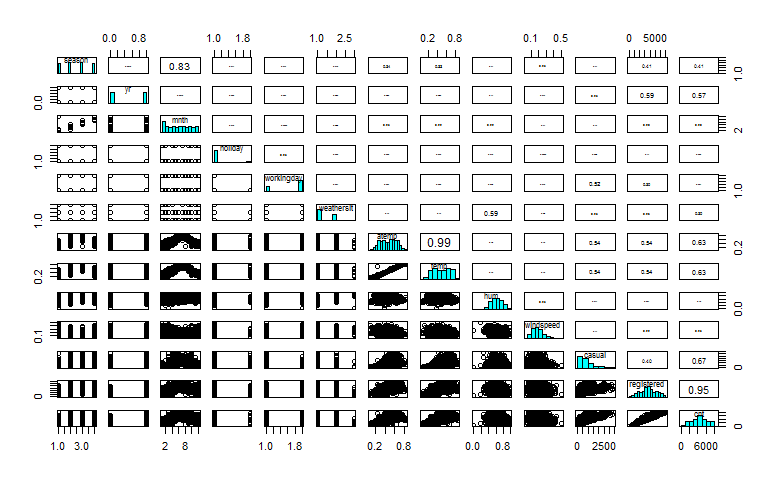
\includegraphics[scale=0.6]{figures/scatterplot.png}
		\label{fig:scatterplot}
		\caption{Scatterplot matrix of bike sharing (daily) dataset}
	\end{figure}
	
	As we can see from Figure \ref{fig:scatterplot}, there are 0.83 correlation between season and mnth, 0.99 correlation between temp and atemp, and 0.95 correlation between registered and cnt, 0.67 between casual and cnt.
	
	High correlation between two variables means that as one variable rises or falls, the other variable rises or falls as well. Since we don't want high correlation in our dataset, we can pick one attribute from each pairs with high correlation.
	
	Moreover, from observing the last three columns of correlation between different attributes to registered, casual, and cnt, we can have a list of the correlations in decreasing order as the following table shows: 
	\begin{table}[H]
		\begin{tabular}{| l | l | l | l | l | l|}
			cnt~ & registered & casual & temp/atemp & yr & season\\
			correlation & 0.95 & 0.67 & 0.63 & 0.57 & 0.41\\
			\hline
			%	registered~ &
		\end{tabular}
	\end{table}
	
	A more clear visualization of correlation can be achieved by a heat map. 
	\begin{figure}[H]
		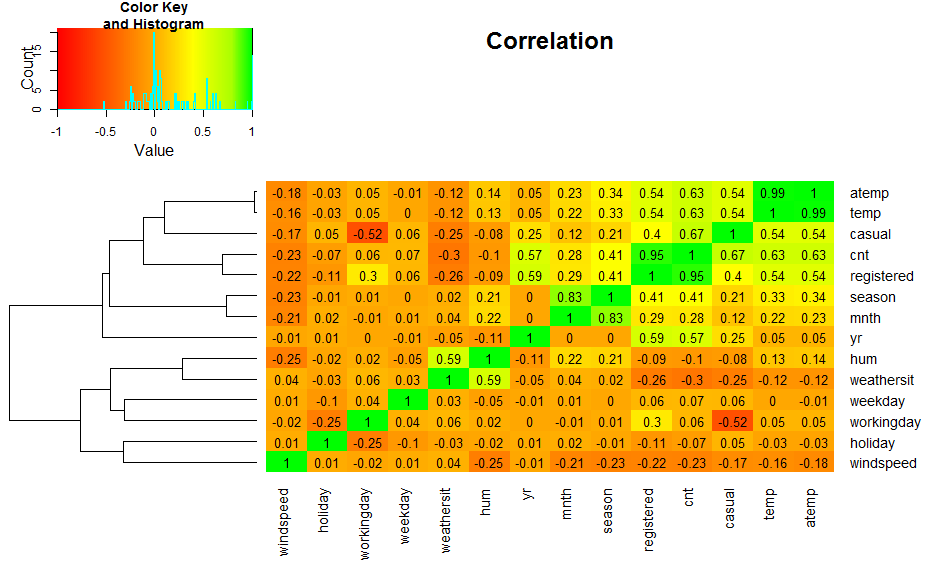
\includegraphics[scale=0.6]{figures/correlation.png}
		\label{fig:correlation}
		\caption{Scatterplot matrix of bike sharing (daily) dataset}
	\end{figure}
	We found that workingday has a negative correlation with casual users from the heat map. 
	Moreover, the heat map has the function of hierarchical clustering. As we can see from left of the above heat map, the clustering put atemp and temp, cnt and registered, season and month, hum and weathersit, weekday and workingday together in the lowest level.  If we cut the hierarchical clustering into two clusters, we will get atemp,temp, casual, cnt, registered, season, mnth, yr as one cluster; hum, weathersit, weekday, workingday, holiday, windspeed as the other cluster.
	
	Another scatterplot matrix on hourly data with random sampling of size 1000 without replacement indicates that the hours have a high correlation with the hourly cnt as we can see from the following figure. 
	\begin{figure}[H]
		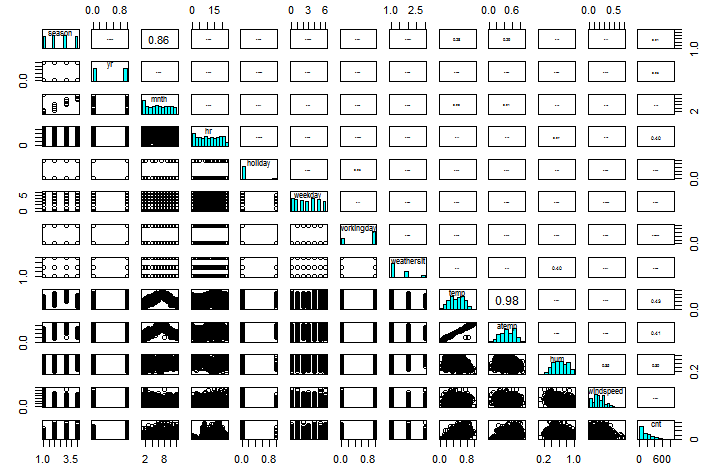
\includegraphics[scale=0.7]{figures/scatterplot_col_season.png}
	\end{figure}
	
	Based on the above observations, we identify that temp, yr, season/mnth, hr, and workingday as our main focus in hourly dataset.
	
	\paragraph*{Explore 1.} Most likely, temperature and weather have correlation with bike demand. We can plot:
	\begin{figure}[H]
		\centering
		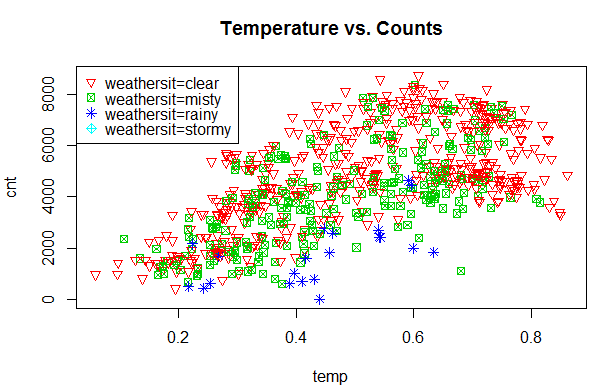
\includegraphics[scale=.85]{figures/temp_counts.png}
	\end{figure}
	
	The rental bike counts increase when the temp increase. Moreover, with the same temperature, the better the weather is, the more bike rental it is.
	
	\begin{figure}[H]
		\centering
		\begin{minipage}{.45\textwidth}
			\centering
			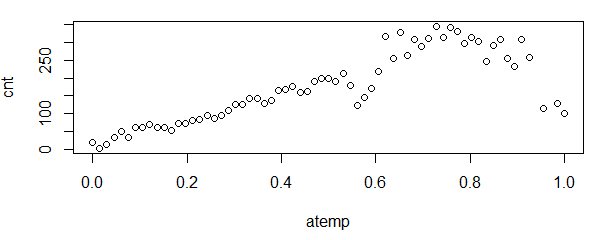
\includegraphics[width=\linewidth]{figures/atemp_cnt.png}
			\caption{Average counts on different atemp}
			\label{fig:atemp}
		\end{minipage}%
		\begin{minipage}{.45\textwidth}
			\centering
			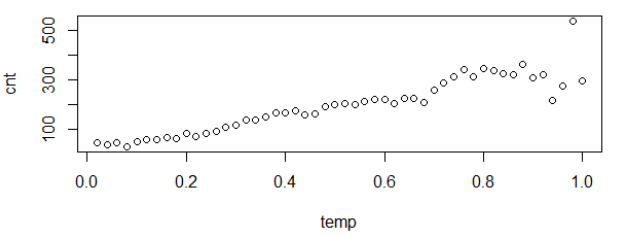
\includegraphics[width=\linewidth]{figures/temp_cnt.png}
			\caption{Average counts on different temp}
		\end{minipage}
	\end{figure}
   We can confirm the rental demand with temp on the above figures. Moreover, we can see from Figure \ref{fig:atemp}, it seems that the bike demand start to decrease when atemp is too high(atemp=0.7). Therefore, we plotted the the bike counts vs. $|atemp-0.7|$, the result is almost linear.
	\begin{figure}[H]
		\centering
		\begin{minipage}{.45\textwidth}
			\centering
			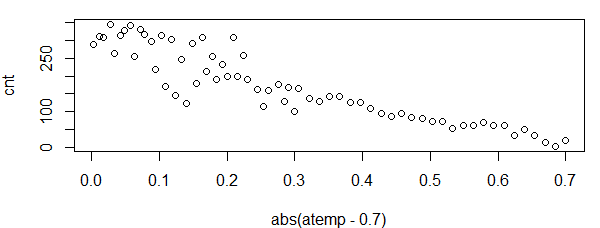
\includegraphics[width=\linewidth]{figures/atemp_abs.png}
		\end{minipage}%
		\begin{minipage}{.45\textwidth}
			\centering
			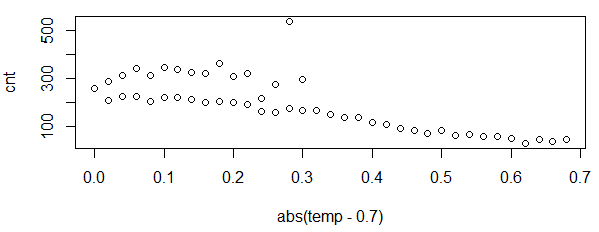
\includegraphics[width=\linewidth]{figures/temp_abs.png}
			%\caption{Average counts on different temp}
		\end{minipage}
	\end{figure}
	
	\paragraph*{Explore 2.} Bike rental vs. weekdays
	Most likely, the bike rental will show a different pattern on weekdays and weekends. part of the people who rent bike on weekdays probably use it for commute to work, people who rent bikes on weekends most likely are for leisure.
	
	First, we plotted the counts on a typical week:
	\begin{figure}[H]
		\centering
		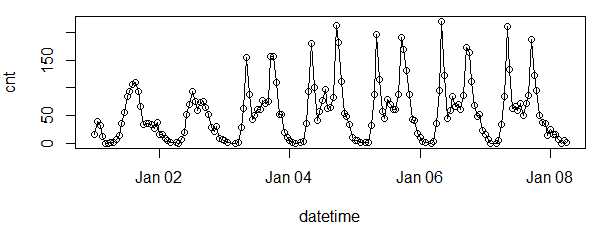
\includegraphics[scale=.8]{figures/week_cnt.png}
	\end{figure}
	
	We see that the bike demand is different on weekdays and weekends in this week. To check if it is true generally, we plotted the average hourly counts conditional on day of the week from the whole dataset.
	\begin{figure}[H]
		\centering
		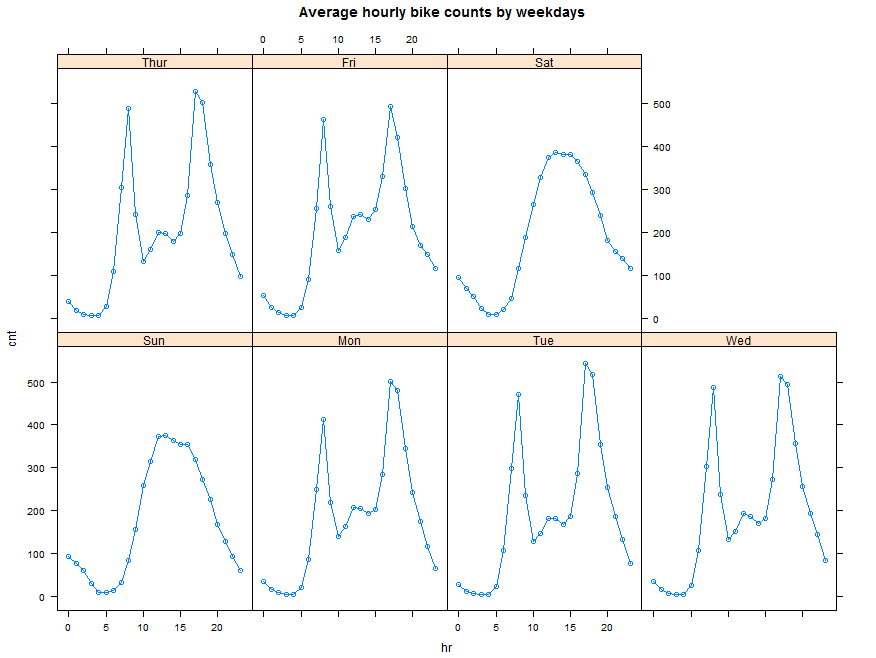
\includegraphics[scale=.6]{figures/hr_weekday.png}
	\end{figure}
	
	The following is the plot of hourly counts conditional on day of the week AND if it's a holiday.
		\begin{figure}[H]
			\centering
			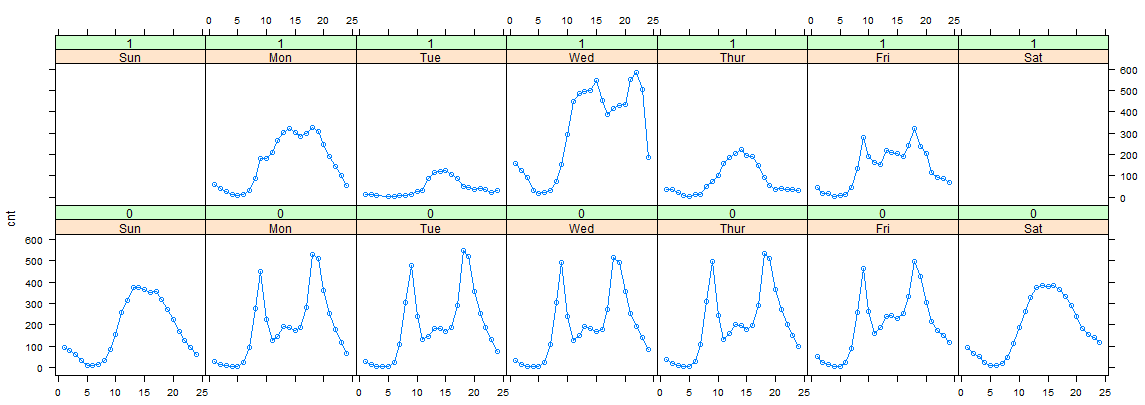
\includegraphics[scale=1]{figures/hr_weekday_holiday.png}
			\caption{Hourly bike rental on different weekdays and holidays (1 indicates holiday, 0 indicates non-holiday)}
		\end{figure}
	From above figure, we can see that whenever there is a holiday, the bike rental shows very different pattern than usual weekdays.  Sometimes the pattern is like a bike rental in weekends (Monday in the above figure).
	
	\paragraph*{Explore 3.} Most certain the hour/workingday of the day also correlates with Bike demand. We can plot: 
	\begin{figure}[H]
		\centering
		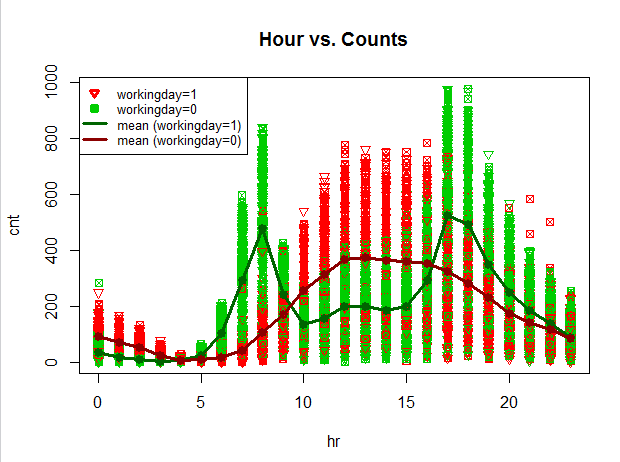
\includegraphics[scale=.85]{figures/hr_cnt.png}
	\end{figure}
	
	As we can see from the above figure, the bike rentals are concentrating from 7am to 7pm. Moreover, the working day and non-working day show a different pattern on bike rental. On workingday, the peak rental occurs at 7-8am, and 5-6pm which is the time people go to work and get off work. On non-workingday, the peak rentals occur from 10am to 4pm, which is the time families do outdoor activity.  From this, a bold guess is that more registered people rent on workingdays, and more casual users rent on non-working days. We confirmed this by the following conditional plot.
	
	
	\paragraph*{Explore 4.} Finally let’s see if usage varies depending on the month\ season. We first drew a boxplot. 
	\begin{figure}[H]
		\centering
		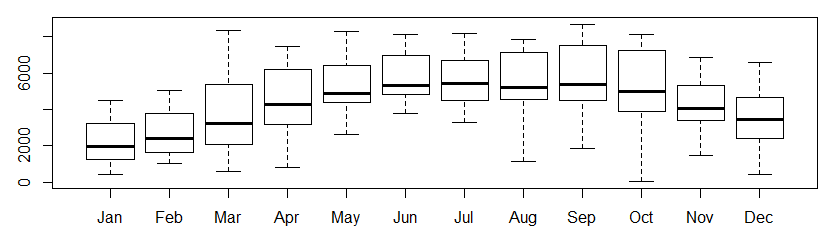
\includegraphics[scale=.6]{figures/month_count.png}
		\caption{Boxplot of counts on different months}
	\end{figure}
	
	We can see that demand in January is the lowest and it peaks in the summer. To explore more, we drew a coplot of hourly bike counts conditioned on month.
	
	\begin{figure}[H]
		\centering
		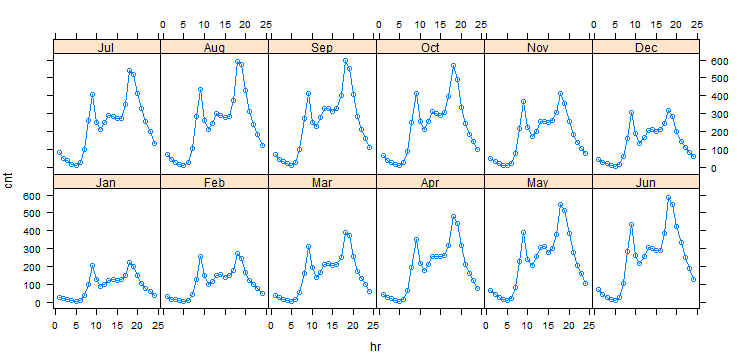
\includegraphics[scale=1]{figures/cnt_hr_mnth.png}
		\caption{Average hourly bike rental on different month)}
	\end{figure}
	The bike rental peaks in the month from May to October. However, the pattern of hourly rental are similar with the peak is bigger in these months. It seems that during the month from May to October, more people rent bikes for commuting to work. For example, compare October and November in the above graph, the rental are very similar except during rush hours. 
	
		\begin{figure}[H]
			\centering
			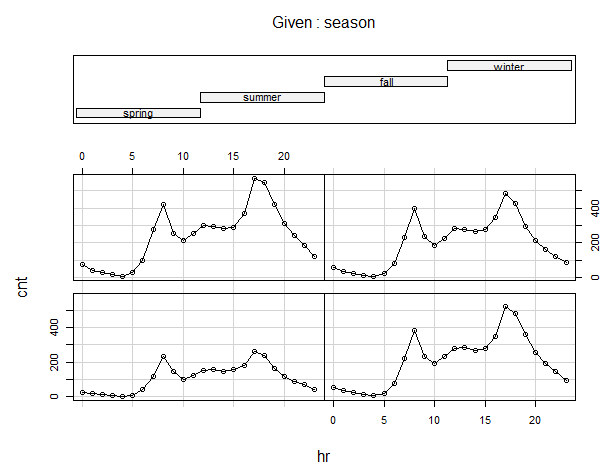
\includegraphics[scale=.9]{figures/coplot_season.png}
			\caption{Coplot of hourly counts conditional on season}
		\end{figure}
	
	 Let's see if different season behave differently by a parallel coordinate plot. The following are the plots from Ggobi for different seasons.
	 
	 \begin{figure}[H]
	 	\centering
	 	\begin{minipage}{.5\textwidth}
	 		\centering
	 		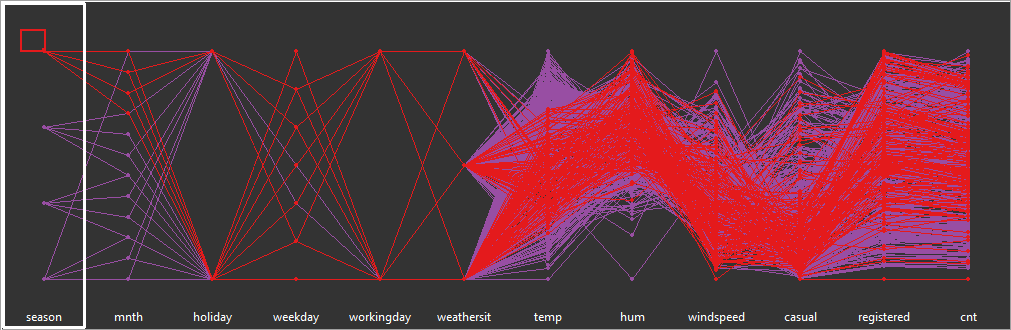
\includegraphics[width=\linewidth]{figures/spring_pcor.png}
	 		\caption{Spring}
	 	\end{minipage}%
	 	\begin{minipage}{.5\textwidth}
	 		\centering
	 		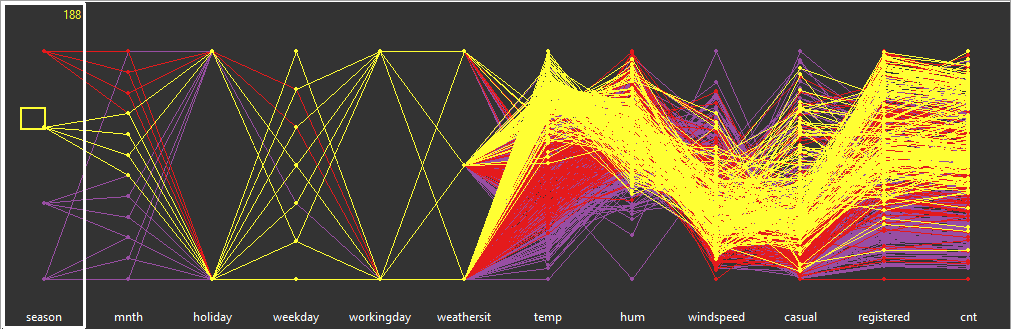
\includegraphics[width=\linewidth]{figures/summer_pcor.png}
	 		\caption{Summer}
	 	\end{minipage}
	 \end{figure}
	 
	 \begin{figure}[H]
	 	\centering
	 	\begin{minipage}{.5\textwidth}
	 		\centering
	 		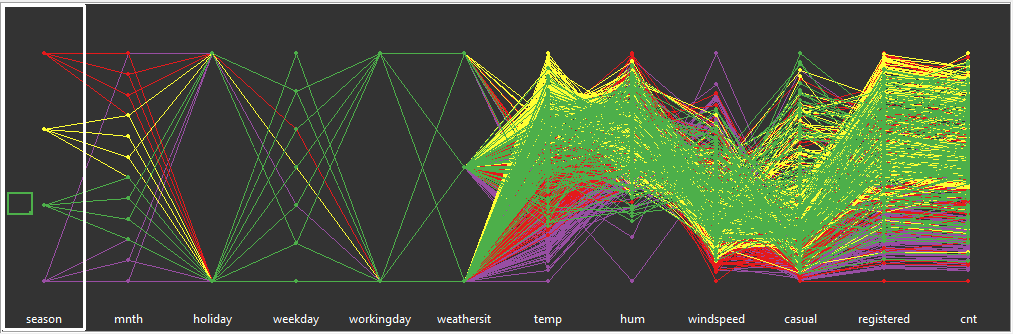
\includegraphics[width=\linewidth]{figures/fall_pcor.png}
	 		\caption{Fall}
	 	\end{minipage}%
	 	\begin{minipage}{.5\textwidth}
	 		\centering
	 		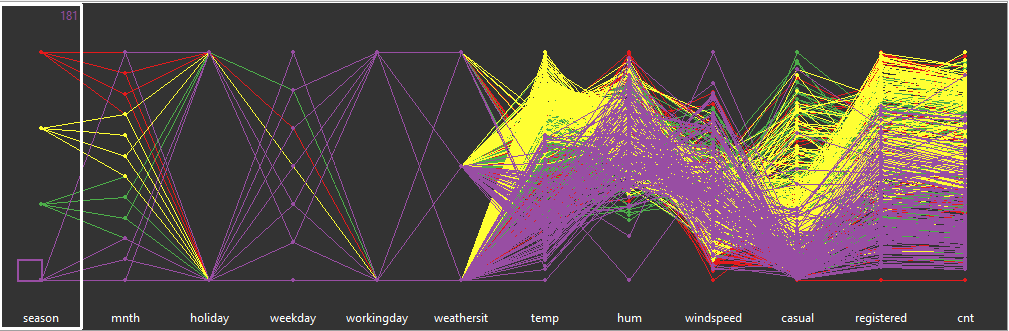
\includegraphics[width=\linewidth]{figures/winter_pcor.png}
	 		\caption{Winter}
	 	\end{minipage}
	 \end{figure}
	From the above plots, we can see that casual/registered users' demand are different in different seasons. The pattern is summarize in the following table. 
	
	\begin{table}[H]
		\centering
		\begin{tabular}{|l|l|l|l|l|}
			\hline
			Season & 	Spring & Summer & Fall & Winter\\ \hline
			Registered & median, high & median, high & median, high & low, median\\
			Casual & low & low, median, high & low, median & low \\ \hline
		\end{tabular}
	\end{table}
	
	
    It seems that month will give more accurate information than season in the prediction. Since these two attributes are highly correlated, we will keep month in our experiment.	
		
	\paragraph*{Explore 5.} Registered and casual users' demand Vs. workingday
	 \begin{figure}[H]
	 	\centering
	 	\begin{minipage}{.5\textwidth}
	 		\centering
	 		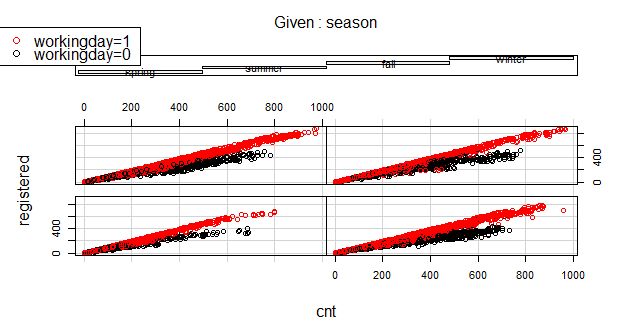
\includegraphics[width=\linewidth]{figures/registered_cnt_season.png}
	 		\caption{registered-cnt$|$season}
	 		\label{fig:registered-cnt}
	 	\end{minipage}%
	 	\begin{minipage}{.5\textwidth}
	 		\centering
	 		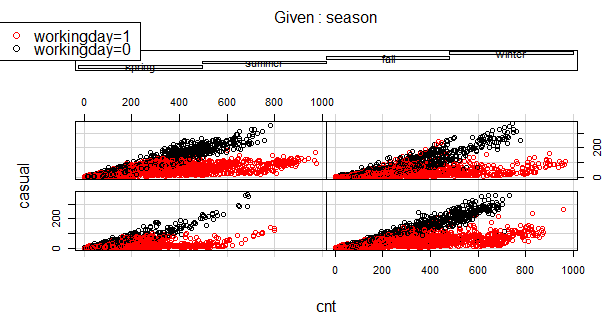
\includegraphics[width=\linewidth]{figures/casual_cnt_season.png}
	 		\caption{casual-cnt$|$season}
	 		\label{fig:casual-cnt}
	 	\end{minipage}
	 \end{figure}
	 From Figure \ref{fig:registered-cnt} and Figure \ref{fig:casual-cnt}, we can see that Registered users and casual users behave differently on workingday. More registered users rent bike on workingdays, and more casual users rent bike on non-working days.
	 	\begin{figure}[H]
	 		\centering
	 		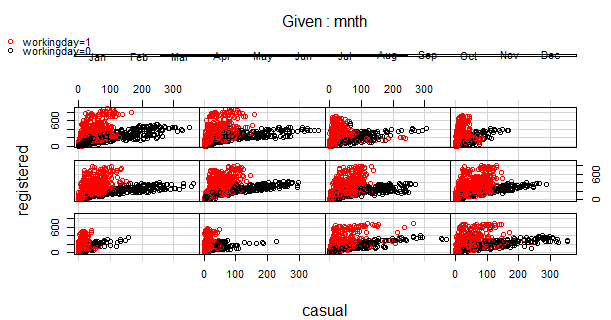
\includegraphics[scale=.9]{figures/coplot_registered_casual_mnth.png}
	 		\caption{Coplot of registered-casual$|$ mnth colored on workingday}
	 	\end{figure}
	In the above graph, on the non-working day, the registered and casual almost have a linear correlation(black dots). However, on workingday, there is no strong linear correlation between the two (red dots). This suggests us that we should build two separated model for workingday and non-workingday.
	
	To find more, we plotted casual and registered for everyday as appendix A shows. Here are some interesting findings for casual users:
	\begin{enumerate}
		\item In winter, less casual users go out on weekdays, but similar amount of users go out during weekend in winter and summer.
	
		 \begin{figure}[H]
		 	\centering
		 	\begin{minipage}{.5\textwidth}
		 		\centering
		 		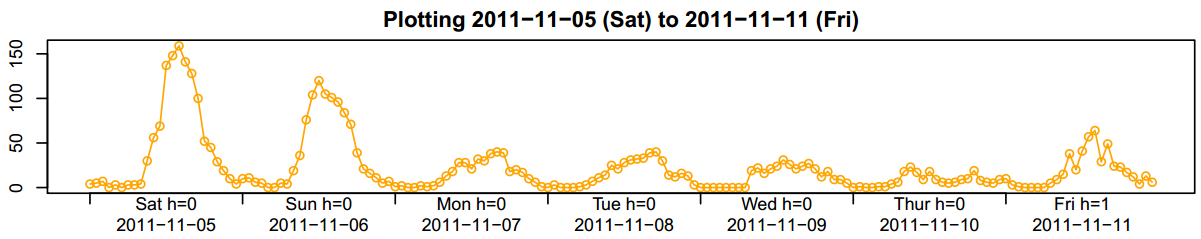
\includegraphics[width=\linewidth]{figures/casual_typical_winter.png}
		 		\caption{casual typical winter}
		 	\end{minipage}%
		 	\begin{minipage}{.5\textwidth}
		 		\centering
		 		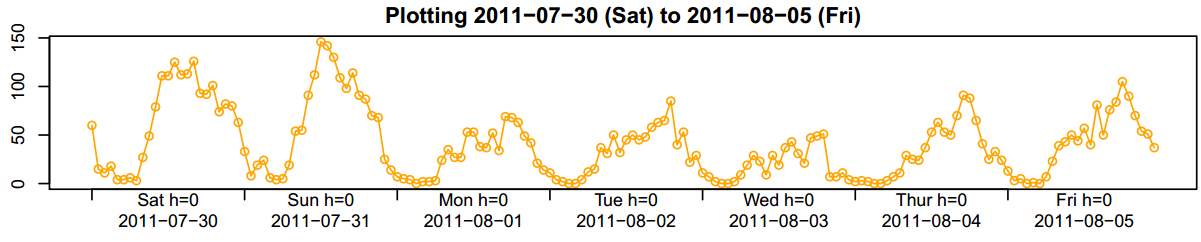
\includegraphics[width=\linewidth]{figures/casual_typical_summer.png}
		 		\caption{casual typical summer}
		 		%\label{fig:casual-cnt}
		 	\end{minipage}
		 \end{figure}
	 \item The week when school started is atypical than usually summer weeks. This indicates that a large percent of casual users might be student.
	 
	 	 \begin{figure}[H]
	 	 	\centering
	 	 	\begin{minipage}{.5\textwidth}
	 	 		\centering
	 	 		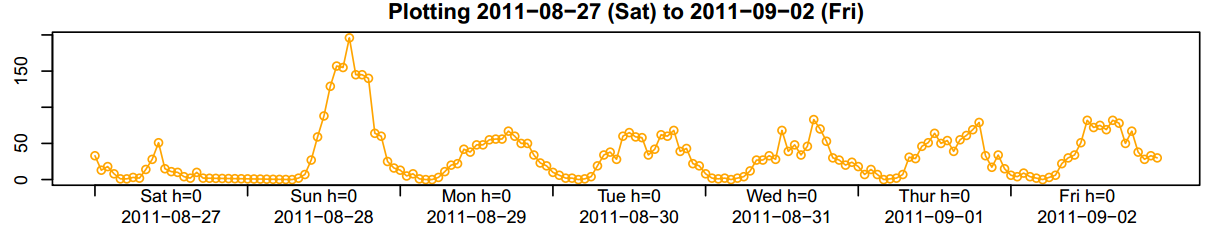
\includegraphics[width=\linewidth]{figures/casual_week_before_school.png}
	 	 		\caption{casual week before school}
	 	 	\end{minipage}%
	 	 	\begin{minipage}{.5\textwidth}
	 	 		\centering
	 	 		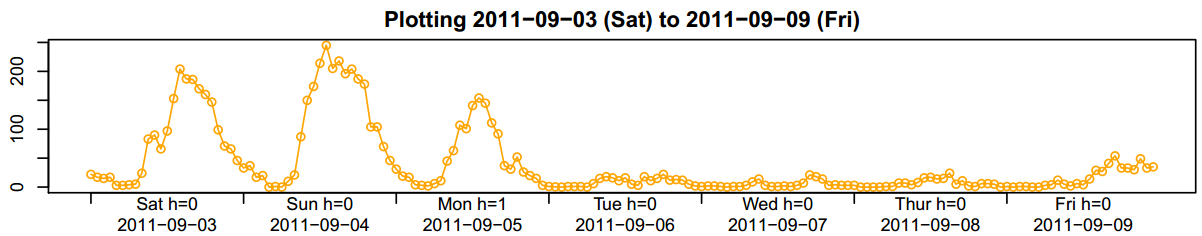
\includegraphics[width=\linewidth]{figures/casual_school_start.png}
	 	 		\caption{casual school start}
	 	 		%\label{fig:casual-cnt}
	 	 	\end{minipage}
	 	 \end{figure}

	\item Christmas is atypical than regular winter weeks.
		 \begin{figure}[H]
		 	\centering
		 	\begin{minipage}{.5\textwidth}
		 		\centering
		 		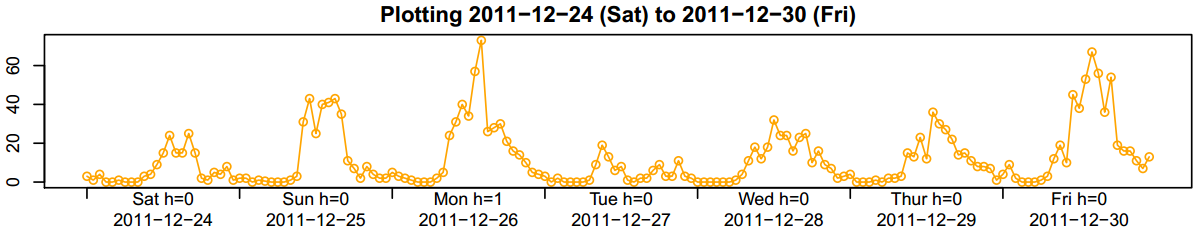
\includegraphics[width=\linewidth]{figures/casual_chritmas_2011.png}
		 		\caption{casual chritmas 2011}
		 	\end{minipage}%
		 	\begin{minipage}{.5\textwidth}
		 		\centering
		 		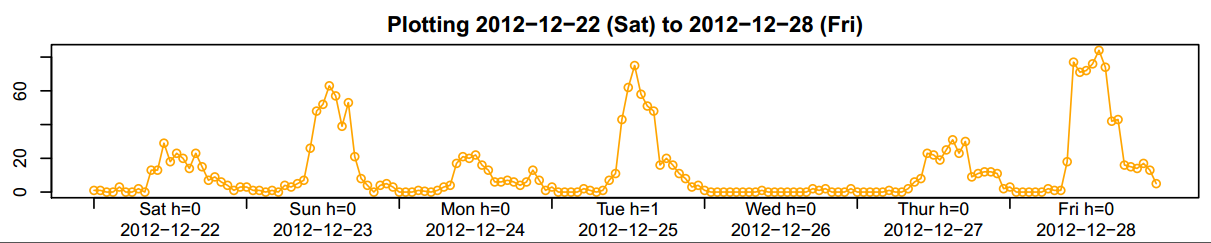
\includegraphics[width=\linewidth]{figures/casual_christmas.png}
		 		\caption{casual christmas 2012}
		 		%\label{fig:casual-cnt}
		 	\end{minipage}
		 \end{figure}
		 
		 \item Typical winter and summer for registered users don't change that much, except more registered users go bike during the weekends in summer.
		 	\begin{figure}[H]
		 		\centering
		 		\begin{minipage}{.5\textwidth}
		 			\centering
		 			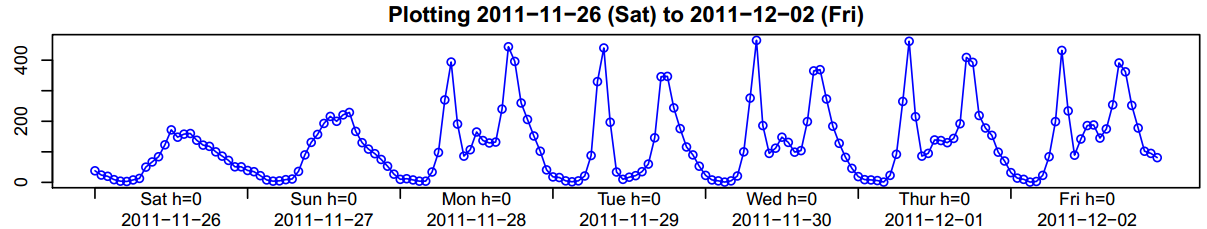
\includegraphics[width=\linewidth]{figures/registered_typical_winter.png}
		 			\caption{registered typical winter}
		 		\end{minipage}%
		 		\begin{minipage}{.5\textwidth}
		 			\centering
		 			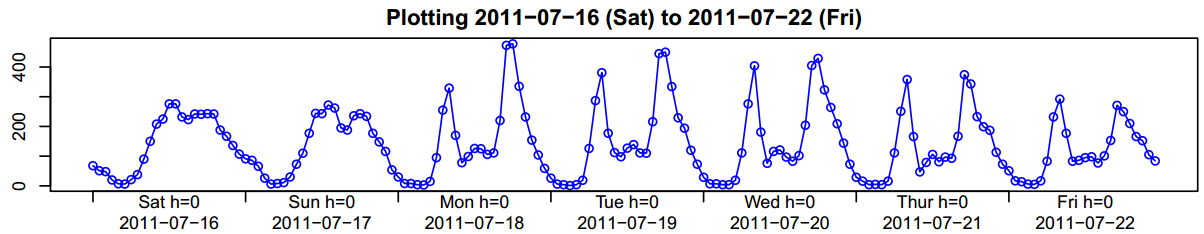
\includegraphics[width=\linewidth]{figures/registered_typical_summer.png}
		 			\caption{registered typical summer}
		 			%\label{fig:casual-cnt}
		 		\end{minipage}
		 	\end{figure}
		 	
		\item Christmas is atypical than regular winter weeks.
			 \begin{figure}[H]
			 	\centering
			 	\begin{minipage}{.5\textwidth}
			 		\centering
			 		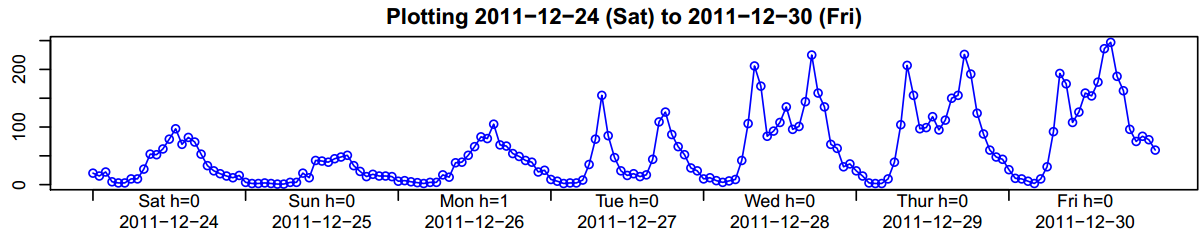
\includegraphics[width=\linewidth]{figures/registered_christmas_2011.png}
			 		\caption{registered chritmas 2011}
			 	\end{minipage}%
			 	\begin{minipage}{.5\textwidth}
			 		\centering
			 		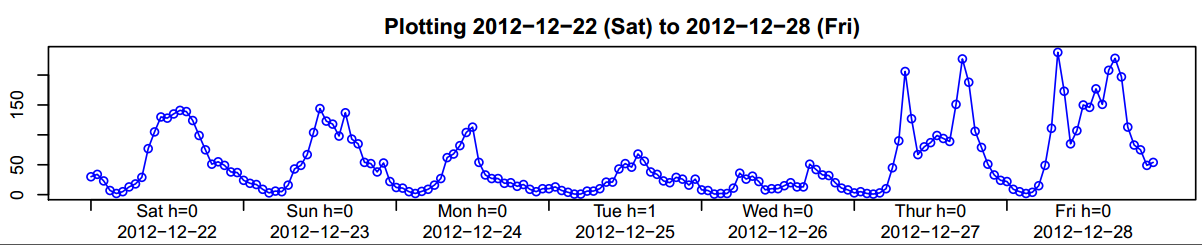
\includegraphics[width=\linewidth]{figures/registered_christmas_2012.png}
			 		\caption{registered christmas 2012}
			 		%\label{fig:casual-cnt}
			 	\end{minipage}
			 \end{figure}
		\end{enumerate}
		
	\paragraph*{Preliminary Conclusion.}In short we have identified strong correlation between counts and with these predictors: 1. Temperature 2. Hour of the Day 3. Working Day 4. Month of the Year. 
	
	\subsection{Association Rule Mining}	
	To investigate more about the dataset, we did an association rule mining. The bike sharing dataset contains a mixture of categorical and numeric attributes and therefore need some preparation before using apriori algorithm on it. Here are the steps for our experiment in association rule mining:
    \begin{enumerate}
    	\item We fist removed the interrelate features: instant, dteday.
    	\item Then we mapped the seven remaining continuous attributes (temp, atemp, hum, windspeed, registered, casual, and cnt) to ordinal attributes by building suitable categories.
    	\item Coerce the data set to transactions as a binary incidence matrix.
    	\item run Apriori algorithm with support = 0.01, confidence = 0.3.
    \end{enumerate}
	
	Ming the rules , and sort the rules by lift with "cnt=high" in the rhs. we obtained the following top 5 rules: \color{blue}
	\begin{verbatim}
	   lhs                   rhs           support confidence     lift
	   1  {weekday=Sat,                                                  
	   casual=high}      => {cnt=high} 0.03283174          1 3.768041
	   2  {casual=high,                                                  
	   registered=high}  => {cnt=high} 0.02872777          1 3.768041
	   3  {hum=medium,                                                   
	   casual=high}      => {cnt=high} 0.03283174          1 3.768041
	   4  {mnth=Sep,                                                     
	   registered=high}  => {cnt=high} 0.03419973          1 3.768041
	   5  {mnth=Jun,                                                     
	   registered=high}  => {cnt=high} 0.03009576          1 3.768041
	\end{verbatim} \color{black}
    The first rule tells us that when it is Saturday and casual counts is high, there will be a large chance that cnt is high.
    
    sort the rules by lift with "registered=high" in the rhs. we obtained the following top 5 rules: \color{blue}
	\begin{verbatim}
	   lhs                rhs                  support confidence     lift
	   1  {weekday=Fri,                                                      
	   cnt=high}      => {registered=high} 0.03967168          1 3.673367
	   2  {weekday=Wed,                                                      
	   cnt=high}      => {registered=high} 0.03693570          1 3.673367
	   3  {weekday=Thur,                                                     
	   casual=medium} => {registered=high} 0.01231190          1 3.673367
	   4  {weekday=Thur,                                                     
	   cnt=high}      => {registered=high} 0.04377565          1 3.673367
	   5  {casual=low,                                                       
	   cnt=high}      => {registered=high} 0.12859097          1 3.673367
	\end{verbatim}\color{black}
	These five rules in general tells us that when it is weekdays, registered is high.
	
	 sort the rules by lift with "casual=high" in the rhs. we obtained the following top 5 rules: \color{blue}
	\begin{verbatim}
	   lhs                   rhs              support confidence     lift
	   1  {season=summer,                                                   
	   weekday=Sat,                                                     
	   cnt=high}         => {casual=high} 0.01504788          1 16.61364
	   2  {season=summer,                                                   
	   weekday=Sat,                                                     
	   workingday=0,                                                    
	   cnt=high}         => {casual=high} 0.01504788          1 16.61364
	   3  {season=summer,                                                   
	   weekday=Sat,                                                     
	   atemp=medium,                                                    
	   cnt=high}         => {casual=high} 0.01094391          1 16.61364
	   4  {season=summer,                                                   
	   yr=2012,                                                         
	   weekday=Sat,                                                     
	   cnt=high}         => {casual=high} 0.01504788          1 16.61364
	   5  {season=summer,                                                   
	   weekday=Sat,                                                     
	   weathersit=clear,                                                
	   cnt=high}         => {casual=high} 0.01231190          1 16.61364
	\end{verbatim}\color{black}
	Here, we can see that when it is summer weekends and cnt is high, there will be a very large chance that casual is high.  
	
	Rule 4 attracted our attention since it indicates that yr=2012 can help to predict high casual bike rental demand. We therefore plotted casual counts on yr 2011 and 2012 to compare the difference. 
	
	The association rule mining didn't give us too much more information about the dataset. But it confirms that Casual and Registered users behave differently. In the summer weekends, there are more bike rentals from casual bikers. In weekdays, there are more bike rentals from registered bikers. 
	
	\begin{figure}[H]
		\centering
		\begin{minipage}{.48\textwidth}
			\centering
			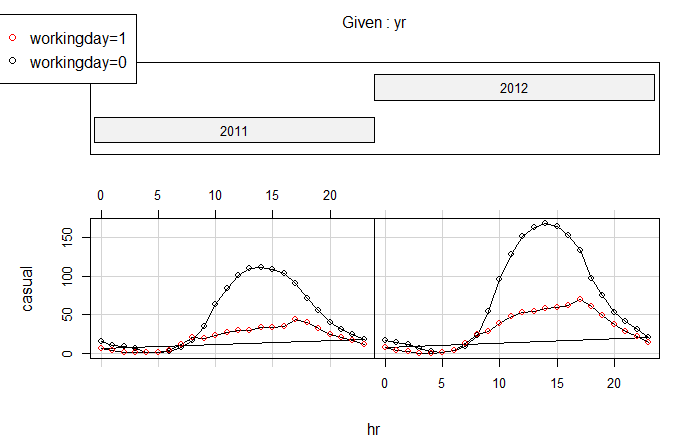
\includegraphics[width=\linewidth]{figures/casual_yr.png}
			\caption{Coplot of casual-hr$|$ yr colored on workingday}
			%\label{fig:registered-cnt}
		\end{minipage}%
		\begin{minipage}{.48\textwidth}
			\centering
			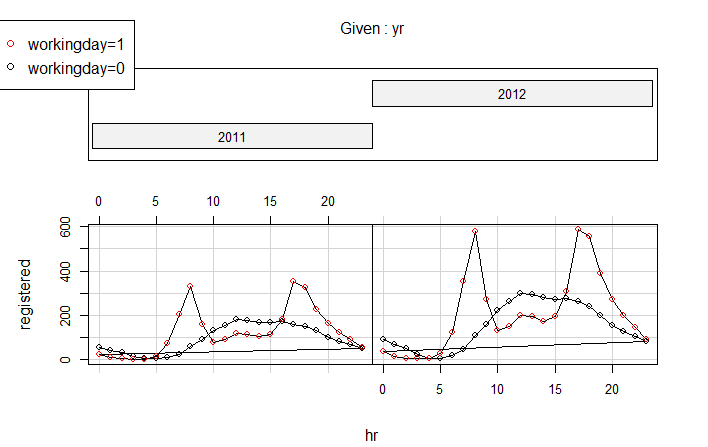
\includegraphics[width=\linewidth]{figures/registered_yr.png}
			\caption{Coplot of registered-hr$|$ yr colored on workingday}
			%\label{fig:casual-cnt}
		\end{minipage}
	\end{figure}
	
		\begin{figure}[H]
			\centering
			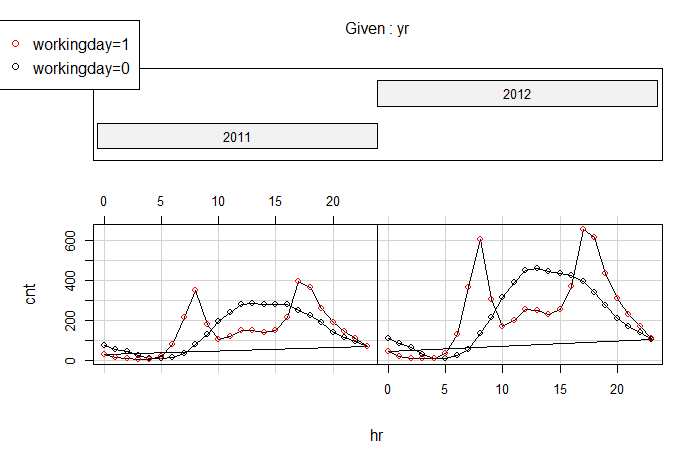
\includegraphics[scale=.8]{figures/cnt_year.png}
			\caption{Coplot of cnt-hr$|$ yr colored on workingday}
		\end{figure}
    From above figures, the bike rental demand from registered users and casual users all increase from 2011 to 2012 without changing on underlying pattern of the rental. Therefore, yr is also a strong predictor in bike sharing dataset.
	\section{Unsupervised Learning: Data Preprocessing}
	\subsection{Dimension Reduction: PCA }
	\label{sec:dimension-reduction}
	
	\subsection{Data Reduction: Clustering Kmeans + Davies-Bouldi Index}
	\label{data-reduction}
	
	The bike sharing dataset has  17365 data instances for the hourly bike sharing dataset. Instead of dimension reduction to reduce the number of attributes, we can use data reduction to reduce the number of cases. In this section, we consider to use clustering methods to cluster together similar cases. By doing so, we can have a reduced representation in volume but produces the same or similar analytical results.
	\subsubsection{Data transformation}
	The k-means clustering uses Euclidean distance to calculate the similarity between instances, therefore the attributes of the input should be continuous numerical values. The bike sharing dataset has a mixture of categorical and numerical values, we thus need some data transformation before running k-means algorithm.
	
	Instead of using all information to clustering the data, we considered only cluster the daily bike rental patterns. We thus feed the cnt to the k-means to group the days with similar cnt pattern together. We thus transformed the cnt in hourly dataset into days by aggregate data into days. Each day has 24 counts from hour 0 to hour 23.  The following is the first 6 instances of the matrix for k-means: \color{blue}
	\begin{verbatim} 
	head(bike.24hourscnt)
 	  hr0 hr1 hr2 hr3 hr4 hr5 hr6 hr7 hr8 hr9 hr10 hr11 hr12 hr13 hr14 hr15
	1  16  40  32  13   1   1   2   3   8  14   36   56   84   94  106  110
	2  17  17   9   6   3  NA   2   1   8  20   53   70   93   75   59   74
	3   5   2  NA  NA   1   3  30  64 154  88   44   51   61   61   77   72
	4   5   2   1  NA   2   4  36  94 179 100   42   57   78   97   63   65
	5   6   6   2  NA   2   3  33  88 195 115   57   46   79   71   62   62
	6  11   4   2  NA   1   4  36  95 219 122   45   59   84   67   70   62
	  hr16 hr17 hr18 hr19 hr20 hr21 hr22 hr23
	1   93   67   35   37   36   34   28   39
	2   76   65   53   30   22   31    9    8
	3   76  157  157  110   52   52   20   12
	4   83  212  182  112   54   48   35   11
	5   89  190  169  132   89   43   42   19
	6   86  172  163  112   69   48   52   23
	\end{verbatim} \color{black}
	The goal is to use k-means and DBI to find a proper way to cluster the dataset. For example, as the following graph shows.
	\begin{figure}[H]
		\centering
		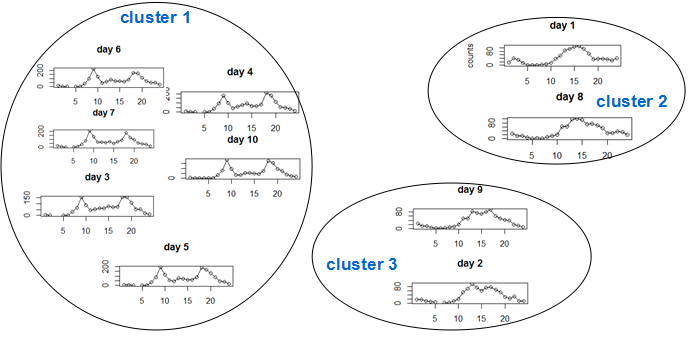
\includegraphics[scale=.8]{figures/cluster_goal.png}
		\caption{One example of k-means goal}
	\end{figure}
	
	
	\subsubsection{Fill in missing values}
	As we can see from last section, the bike sharing dataset has lots of missing values. For example, the bike counts on the second day at hour 5 is missing. A check shows that there are 76 days with missing values, 14 days with more than 1 missing values. 
	
	We can fill up the missing values by three ways with the ``zoo'' package:
	\begin{enumerate}
		\item fill the missing value by last 
		
		\item fill the missing value by linear 
		
		\item fill the missing value by cubic spline	
	\end{enumerate}
	We remove the data of hour(3,5,6,10,11,15,16) on day 1 and day 10, and fill them with the three filling methods. Then we computed the Root Mean Square Error. 
	\begin{figure}[H]
		\centering
		\begin{minipage}{.45\textwidth}
			\centering
			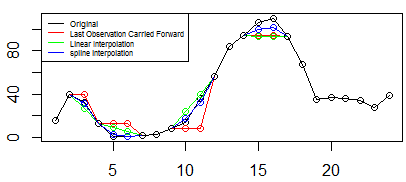
\includegraphics[width=\linewidth]{figures/day1_missing_value.png}
			\caption{ 3 filling methods on day 1,  rmse(locf)=8.093207, rmse(linear)=5.273207, rmse(spline)=2.306192}
			%\label{fig:registered-cnt}
		\end{minipage}%
		\begin{minipage}{.42\textwidth}
			\centering
			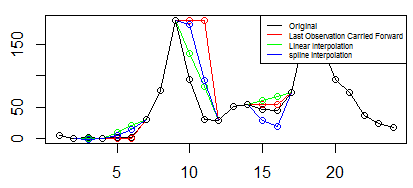
\includegraphics[width=\linewidth]{figures/day10_missing_value.png}
			\caption{ 3 filling methods on day 10, rmse(locf)=37.4316, rmse(linear)=15.07681, rmse(spline)=22.98093}
			
			%\label{fig:casual-cnt}
		\end{minipage}
	\end{figure}
 From the rmse on workingday and non-working days, we found linear or spline interpolation fits our dataset better. We chose a combination of linear and spline interpolation to fill the whole dataset, we first used spline to fill the dataset, then the rest miss values are filled by linear interpolation.
\subsubsection{k-means}	

After we filled up the missing values, we performed k-means from 2 to 9 clusters. The following is the plot of these clusters with the first two principle components as the axis.
	\begin{figure}[H]
		\centering
		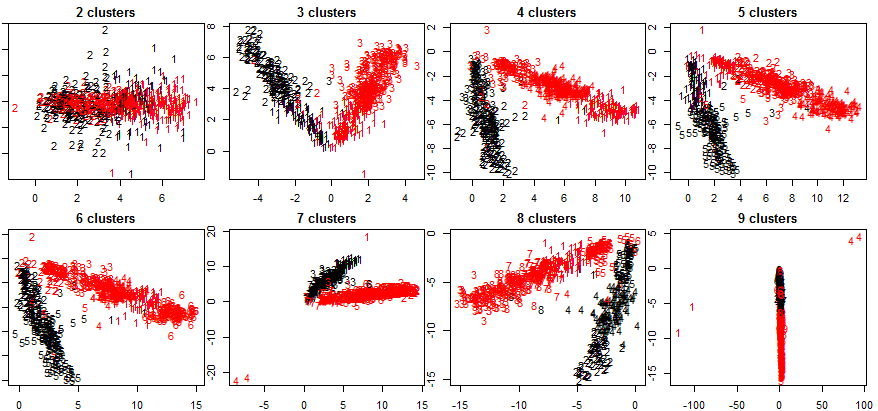
\includegraphics[scale=.65]{figures/kmeans_workingday.png}
		\caption{2 to 15 clusters with DBI with color=red on workingday and black on non-workingday}
	\end{figure}

We can see that workingday give a good separation in 3,4,5,6,7,8 clusters. To investigate what's other attributes the clustering used to 	separate the data. we print out the average temperature on each cluster.

Let's use k=4 as an example: \color{blue}
\begin{multicols}{2}
	\begin{verbatim}
Cluster #1
Working days: 246 (100%)
Total days: 246
Cluster #2
Working days: 107 (53.8%)
Total days: 199
Cluster #3
Working days: 4 (2.84%)
Total days: 141
Cluster #4
Working days: 143 (98.6%)
Total days: 145
	\end{verbatim}
	\columnbreak
	\begin{verbatim}
Cluster #1
Avg temperature: 0.4974
Total days: 246
Cluster #2
Avg temperature: 0.3197
Total days: 199
Cluster #3
Avg temperature: 0.5463
Total days: 141
Cluster #4
Avg temperature: 0.5776
Total days: 145
	\end{verbatim}
\end{multicols} 
\color{black}
As we can see, cluster 1 and 4 are mainly composed of workingdays: 100\% in cluster 1, 98.6\% in cluster 4; cluster 3 are mainly composed of non-working days (97.26\%).  Cluster 2 is a mixture of working and non-workingday, But the temperature in cluster 2 is obviously lower than other clusters(most likely to be in the winter). Therefore, workingday and temp are good attributes for this clustering separation.

A drawing on average counts on each cluster confirmed our finding:
	\begin{figure}[H]
		\centering
		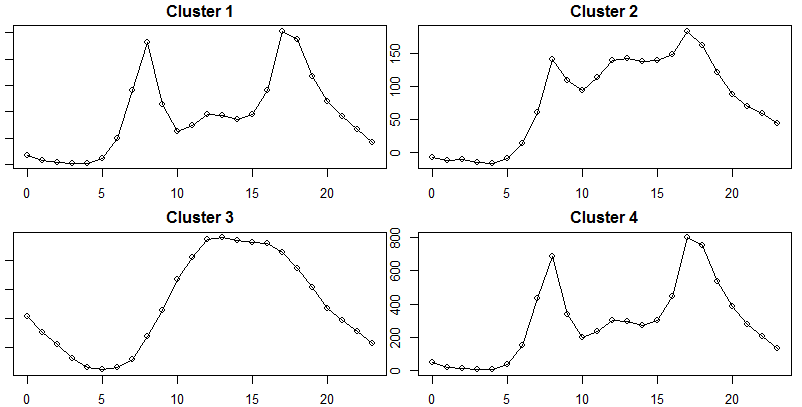
\includegraphics[scale=.65]{figures/kmeans_clusters.png}
		\caption{Average counts plot on each cluster}
	\end{figure}
The following are the findings:

\begin{enumerate}
	\item cluster 1 and cluster 4 are having the pattern of workingdays. However, the counts in cluster 1 is lower than cluster 4 which indicates cluster 1 is representative for lower temp, and 4 for higher temp.
	item counts in cluster 2 look like a mixture of working and non-working days with low counts. It is more likely in the winter.
	\item cluster 3 are high counts with non-working day pattern.
\end{enumerate}

\subsubsection{DBI}
To determine how many clusters we should choose for the k-means, we used Davies-Bouldin index method. After 8 runs, we find the following graph is representative with the averaged minimum DBI=8.
	\begin{figure}[H]
		\centering
		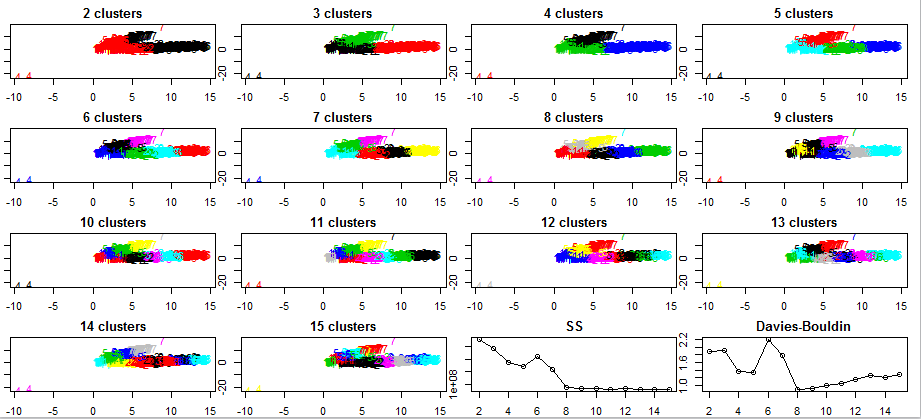
\includegraphics[scale=.65]{figures/dbi_8.png}
		\caption{2 to 15 clusters with DBI}
	\end{figure}
	
	\subsection{Data Reduction: Outlier Detection}
	Another way to reduce the data is getting rid of extreme values. By doing so, we can find a better representation of the data. In this section, we consider to use Interquartile Range ( ``A filter for detecting outliers and extreme values based on interquartile ranges.'') in WEKA  and lofactor in R to detect outliers.  
	
	We first tried Interquartile Range in WEKA. However, this ``smart'' algorithm gave us 21 outliers which are all holidays:
		\begin{figure}[H]
			\centering
			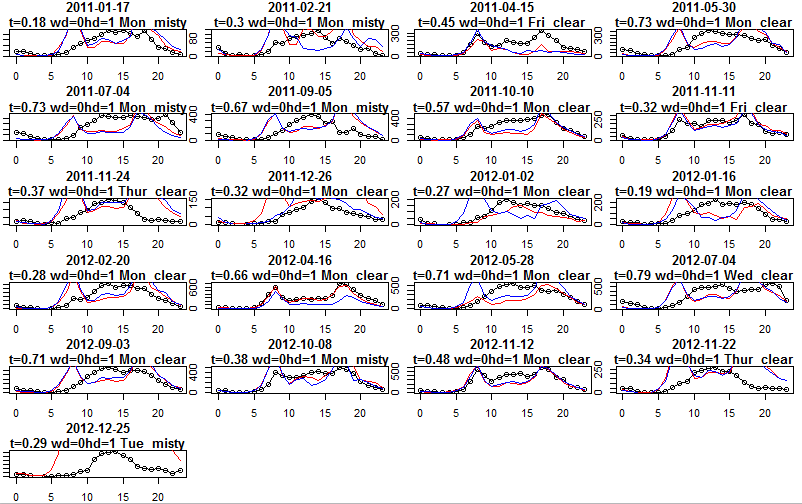
\includegraphics[scale=.65]{figures/outlier_weka_holliday.png}
			\caption{outliers detected by WEKA (black line is the count in this day, red is 7 days ago, black is 7 days after)}
		\end{figure}
	We can see that the black lines are very different than red lines (7 days ago) and blue lines (7 days after)	in all 21 days. This is because all of these 21 holidays are happening during the weekdays. In holiday, the pattern is the non-workingday. And these holidays usually happen in weekdays.
	
	We decided to remove the holiday information in the dataset, and ran Interquartile Range filter again on the dataset. Then we obtained the following days as outliers:
		\begin{figure}[H]
			\centering
			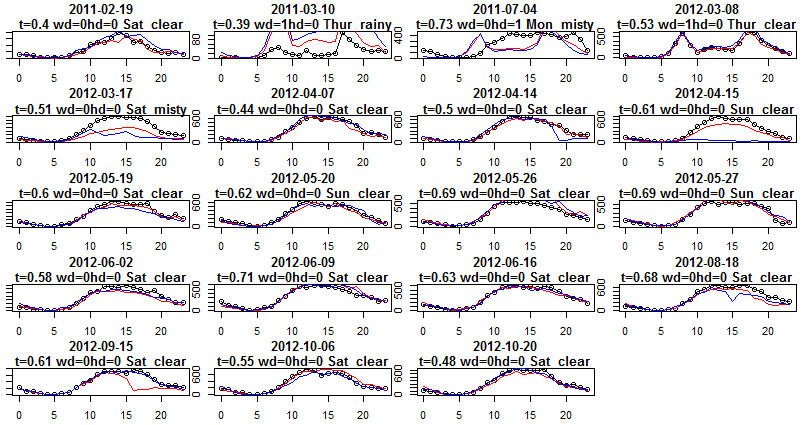
\includegraphics[scale=.65]{figures/outlier_weka_nonholliday.png}
			\caption{outliers detected by WEKA without holiday information}
		\end{figure}
	It seems that only on 2011-03-10 and 2011-07-04, the black lines are different than red/blue lines.
	\begin{figure}[H]
		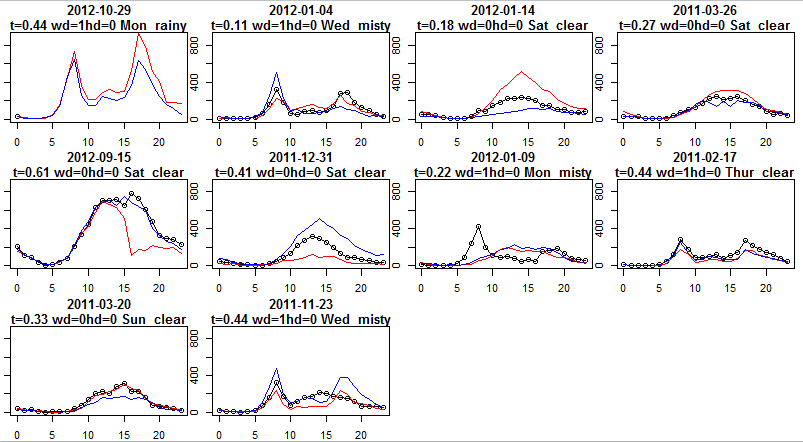
\includegraphics[scale=0.7]{figures/outlier_R.png}
	\end{figure}
 Notice that  on 2012-10-29, there is a big storm based on Gama's paper about event detection \cite{dataset}, the detector in R caught this. We use the events detected in Gama's paper as a baseline comparison here. 

 	\begin{figure}[H]
 		\centering
 		\begin{minipage}{.48\textwidth}
 			\centering
 			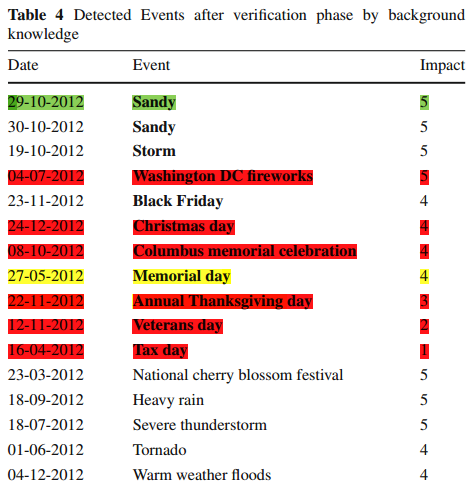
\includegraphics[width=\linewidth]{figures/event_Gama1.png}
 			%\label{fig:registered-cnt}
 		\end{minipage}%
 		\begin{minipage}{.48\textwidth}
 			\centering
 			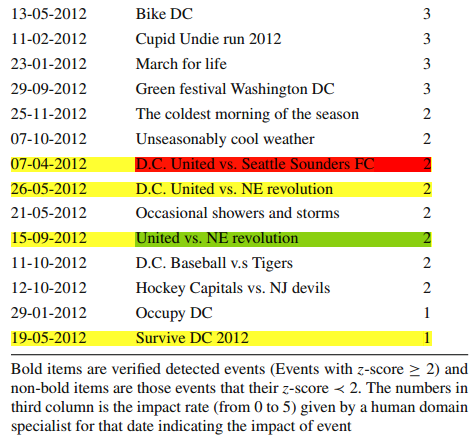
\includegraphics[width=\linewidth]{figures/event_Gama2.png}
 			%\caption{Coplot of registered-hr$|$ yr colored on workingday}
 			%\label{fig:casual-cnt}
 		\end{minipage}
 		5\caption{red: events found by detector 1, yellow: events found by detector 2, green: events found by detector 3}
 	\end{figure}
 	As we can see from the above table, our outlier detectors do help find some events which influence the bike rental. We can eliminate these days found by the three outlier detectors. However, we are also removing points which might be useful since there might be a lot of false alarms on the days detectors found.  
 	
 	A better way to approach is separate data into day of events or not and train models separately on these two datasets. When a new data instance come, we first let the detector decide if it is event day, and pass it to correct model.
	
\section{Experimental Design}
\label{sec:experimental-design}


\section{Experiments and Results}
\label{sec:experiments-and-results}

\section{Supervised Learning}
\label{supervised learning}

The most obvious supervised learning task is to predict \texttt{cnt}, which is a regression problem, since \texttt{cnt} is a continuous variable. This has practical applications, as any company managing a bicycle sharing system might be interested in having a predictive models that helps ensure the supply of bicycles is always appropriate.

\subsection{Kaggle Competition}

The UCI Bike Sharing Dataset is featured as a Kaggle problem called \emph{Bike Sharing Demand}\footnote{\url{www.kaggle.com/c/bike-sharing-demand}}. We decided to participate in the competition, so that we could compare the performance of our method with others.

The competition started on 28 May 2014 and ends on 29 May 2015. As of 13 April 2015, approximately 2900 people or team have participated in this competition, submitting more than 26000 entries.

The Bike Sharing dataset provided by Kaggle is essentially the same as UCI's -- there are only minor differences in the format, such as the date and hour being specified by only one column named \texttt{datetime} and non-normalized units used for temperature, humidity and wind speed.

The data must be split into a training set and a testing set, where the training set is comprised of the first 19 days of every month and the testing set is comprised of the 20th day until the end of the month.

The objective of the competition is to train a classifier on the training data and to predict the testing data's \texttt{cnt} field with the lowest possible root-mean-squared-logarithmic error (RMSLE).

Users can submit their predictions online and the RMSLE will be calculated

Note that the testing data on Kaggle excludes the \texttt{cnt} field. As such, users must submit their predictions only to discover its RMSLE. However, the full data is present in the UCI's dataset and so, we can compute the RMSLE of our predictions by ourselves.

\section{Data preparation}
WILL MOST LIKELY NEED TO MOVE THIS SOMEWHERE ELSE AND JUST REFER TO IT HERE.

The relationship between \texttt{atemp} and \texttt{cnt} is non-linear, as can be seen from GRAPHREF. However, there seems to be a peak temperature for bike rentals at around PEAKTEMP. Hence, it would make sense to define a new variable corresponding to the (absolute value) difference between the current temperature and this ``ideal temperature''. Let \texttt{atempdiff} be defined as:
\begin{verbatim}
atempdiff <- abs(atemp - PEAKTEMP)
\end{verbatim}
Then, the relationship between \texttt{atemptdiff} and \texttt{cnt} is roughly linear as we can see from OTHERGRAPH.

IDEM with \texttt{hum}, except the ``ideal humidity'' is at around 0.2.

\section{Data Imputation}

We observed that some rows are missing in the hourly Bike Sharing datasets. In total, 165 rows are missing, which is almost 7 days worth of data. We decided that it would be wise to impute the missing data, since it could help build a better regression model. Moreover, having no missing data make the R programming significantly easier since the dataset structure would become more regular.

We decided to use the \texttt{zoo} package to handle data imputation. The numeric variables were imputed using linear interpolation. We estimated that this was sufficient for most variables such as temperature, humidity and windspeed. However, for \texttt{casual}, \texttt{registered} and \texttt{cnt}, this did not always work. In most cases, only 1 or 2 observations were missing in a 24-hour period, in which case the linear interpolation was appropriate. However, there are 8 days with a large number of missing observations (between 6 and 23 missing observations per 24-hour period). We decided to investigate visualize the results of our imputation method for those days (see Figure~\ref{fig:badrows}).
\begin{figure}[H]
	\centering
	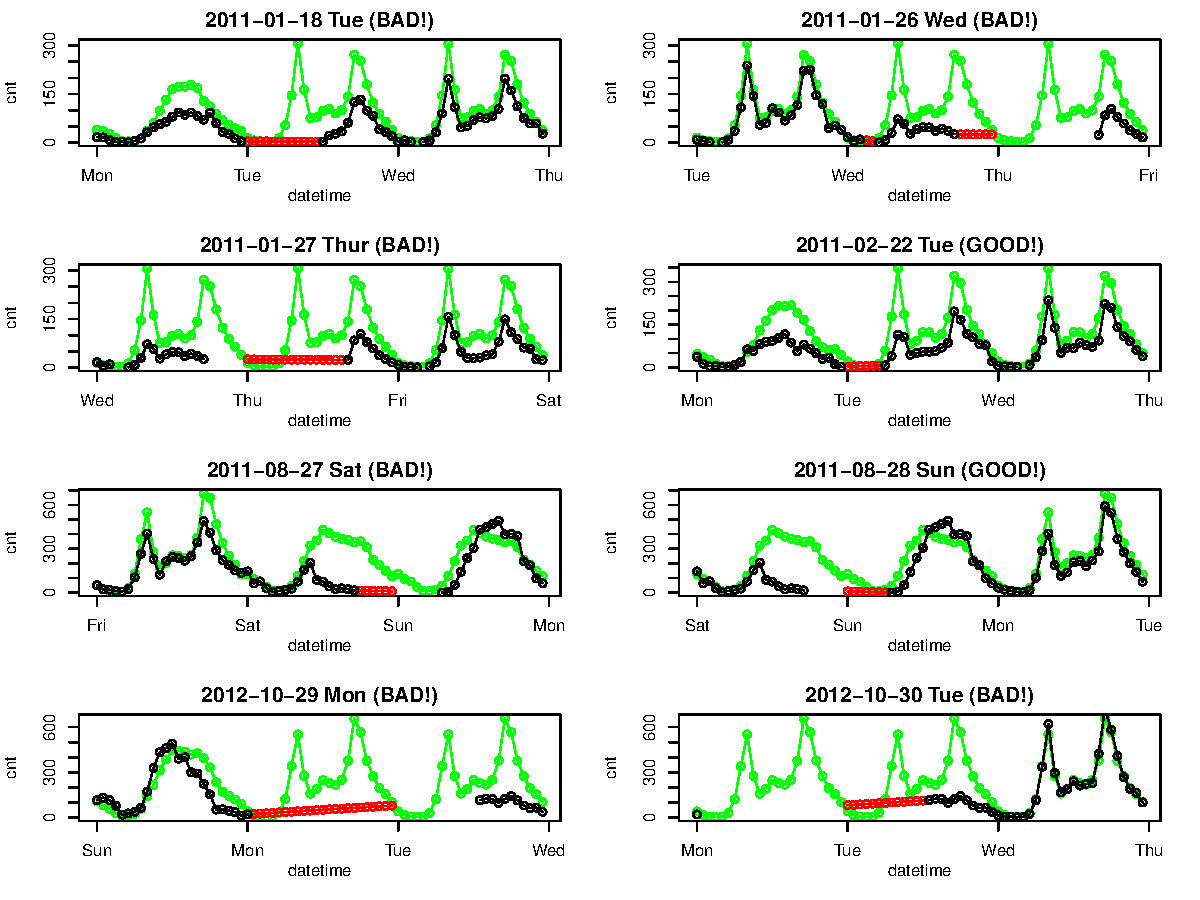
\includegraphics[width=.98\textwidth]{figures/badrows.pdf}
	\caption{Imputation of missing observations for the 8 days with the highest number of missing observations. The {\textbf{\color{black}black}} curve represents the actual values of \texttt{cnt} from the dataset. The {\textbf{\color{red}red}} curve are the observations that were imputed using linear interpolation. The {\textbf{\color{green}green}} curve represents the average value of \texttt{cnt} at the same hour on the same day of the week over the same month (the {\textbf{\color{green}green}} curve therefore provides a rough idea of what a typical day looks like and helps us decide if the imputation is acceptable or not).}
	label{fig:badrows}
\end{figure}
As you can see, in most cases, linear interpolation does a poor job. Indeed, there are too many missing values and the pattern they cover is expected to be highly non-linear, except for the dates 2011-02-22 and 2011-08-28, in which the missing observations are all at night, where the pattern of bikes rental is flat.

At this point, we decided to flag the 6 days above with poor imputation results as ``bad rows''. This allows us to exclude those days completely in the training phase of supervised learning.

\subsection{The two alternative problems on Kaggle}

Unfortunately, the problem of modeling and predicting bike rental demand as stated on Kaggle as two different interpretations.



\section{Conclusion and Further Work}
	\label{sec:conclusion}
	
	
	
\begin{thebibliography}{9}
		\bibitem{dataset}
		Fanaee-T, Hadi, and Gama, Joao, 'Event labeling combining ensemble detectors and background knowledge', Progress in Artificial Intelligence (2013): pp. 1-15, Springer Berlin Heidelberg.
	\end{thebibliography}
	
	>>>>>>> Stashed changes
\end{document}
